% Source: Wald GR, physical PDF pp. 161--171
%         (printed pp. 148--158).
% Coverage: Section 6.4, The Kruskal Extension; equations (6.4.1)--(6.4.32).
% Figures/tables/footnotes: Figs. 6.8--6.12; footnotes 8--9; no tables.
% Status: source-reviewed and compile-clean.
% Uncertainties: none.

\subsection{The Kruskal Extension}\label{sec:6.4}

We turn our attention now to the analysis of the singularities at \(r=2M\) and
\(r=0\) in the coordinate basis components of the metric of the Schwarzschild
solution. As discussed in Section~\ref{sec:6.2}, for any static equilibrium
configuration the region \(r\leq2M\) will be within the matter-filled interior,
so analysis of the singularities at \(r=2M\) and \(r=0\) for the vacuum
Schwarzschild solution is irrelevant to the study of the gravitational field of a
static star, as was first pointed out by Schwarzschild. However, as mentioned at
the end of Section~\ref{sec:6.2}, sufficiently massive bodies will undergo
complete gravitational collapse, and the region \(r\leq2M\) of the vacuum
Schwarzschild solution is very relevant to the description of the endpoint of
this collapse.

Whenever the metric components in a coordinate basis are badly behaved for
certain values of the coordinates, there are two possible causes: (1) The
spacetime geometry is, in fact, singular; or (2) the spacetime geometry is
nonsingular, but the coordinates fail to properly cover a region of spacetime. In
general, it is not an easy task to determine in a given situation which of these
two possibilities holds. (Indeed, it is nontrivial even to formulate a precise
general definition of the notion of singularity in the spacetime geometry. We will
postpone a full discussion of this issue until Chapter~9.) Normally, possibility
(1) would be demonstrated by calculating a curvature scalar, such as
\(R_{abcd}R^{abcd}\), and showing that it blows up at the singularity of the
metric components and furthermore, that this singularity lies at a finite affine
parameter along some geodesic (so that the singularity is not at infinity, in
which case it is not really a singularity). However, as discussed in Chapter~9,
one may have spacetime singularities where no curvature scalars blow up.
Normally, possibility (2) would be demonstrated by explicitly displaying an
extension of the nonsingular region of the original metric, i.e., a nonsingular
spacetime \((\hat M,\hat g_{ab})\) which includes the original spacetime
\((M,g_{ab})\) as a proper subset. Normally, this would be accomplished by finding
a coordinate transformation which eliminates the singularities of the original
metric components.

In the case of the Schwarzschild metric, we already pointed out that the
Schwarzschild coordinates will be badly behaved where the timelike Killing field
\(\xi^a\) becomes collinear with \(\nabla_a r\). We shall see below that this
occurs at \(r=2M\), and that the singularity at \(r=2M\) is merely a coordinate
singularity. On the other hand, the singularity at \(r=0\) is a true singularity
in the spacetime geometry, as can be demonstrated by calculating via
Eqs.~\eqref{eq:6.1.29}--\eqref{eq:6.1.34} the curvature invariant
\(R_{abcd}R^{abcd}\).

We begin, however, by considering two simple examples which help illuminate the
nature of the problem. As a first example, consider the two-dimensional metric
\begin{equation}
  ds^2=-\frac{1}{t^4}dt^2+dx^2
  \tag{6.4.1}\label{eq:6.4.1}
\end{equation}
defined over the coordinate range \(-\infty<x<\infty\), \(0<t<\infty\). This
metric appears to have a singularity at \(t=0\). However, the true nature of the
spacetime geometry can be seen by making the coordinate transformation
\(t\mapsto t'=1/t\). In the new coordinates, the metric is seen to be simply the
flat metric,
\begin{equation}
  ds^2=-(dt')^2+dx^2,
  \tag{6.4.2}\label{eq:6.4.2}
\end{equation}
and the original spacetime is seen to be the portion \(t'>0\) of Minkowski
spacetime. Thus, the apparent singularity at \(t=0\) of the original metric,
Eq.~\eqref{eq:6.4.1}, really represents \(t'\to\infty\) in Minkowski spacetime
and is not a singularity at all but merely corresponds to the covering of an
infinite region of spacetime with a finite range of a coordinate. The spacetime
geometry is geodesically complete as \(t\to0\) (\(t'\to\infty\)), i.e., all the
geodesics approaching \(t=0\) extend to arbitrarily large values of their affine
parameter. On the other hand, the spacetime of Eq.~\eqref{eq:6.4.1} is \emph{not}
geodesically complete as \(t\to\infty\) (\(t'\to0\)). However, we can extend the
original spacetime beyond \(t=\infty\) by adding on the portion \(t'\leq0\) of
Minkowski spacetime. This example provides an excellent illustration of how one
can be misled by interpreting coordinate labels such as \(t\) as physically
meaningful quantities. It also illustrates how an appropriate coordinate
transformation can help one analyze what is really going on in the spacetime.

Our second example will be seen to be closely analogous to the Schwarzschild
solution, and for this reason we will analyze it in detail. We consider the
\emph{Rindler spacetime},
\begin{equation}
  ds^2=-x^2dt^2+dx^2
  \tag{6.4.3}\label{eq:6.4.3}
\end{equation}
with coordinate ranges \(-\infty<t<\infty\), \(0<x<\infty\). This metric
appears to have a singularity at \(x=0\). (The determinant of \(g_{\mu\nu}\)
vanishes at \(x=0\), so the inverse metric components \(g^{\mu\nu}\) are singular
at \(x=0\).) Geodesics terminate with finite length at \(x=0\), but calculation
of curvature scalars shows no bad behavior\footnote{In fact, the curvature of the
Rindler metric vanishes, showing immediately that the Rindler spacetime must be
simply a portion of two-dimensional Minkowski spacetime. However, in order to
pursue the analogy with the Schwarzschild metric, we prefer not to make use of
this fact in our analysis.} as \(x\to0\), suggesting that the singularity may be
simply a coordinate singularity. This metric is not simple enough for trial and
error guesses at coordinate transformations to have much chance of success, so we
need a more systematic approach. In general, the best procedure is to introduce
new coordinates which are linked closely to the spacetime geometry. This can be
achieved, for example, by introducing a family of geodesics which head toward the
singularity and using the affine parameter along the geodesics as one of the
coordinates. In general, there is no foolproof method for elimination of
coordinate singularities; for example, for coordinates based on a family of
geodesics, new coordinate singularities will be produced whenever the geodesics
cross. However, in two-dimensional spacetimes, there does exist an essentially
foolproof method of analyzing coordinate singularities. This is because in two
dimensions, the null geodesics divide up (at least locally) into two classes,
ingoing and outgoing, and within each class two distinct null geodesics cannot
cross, since their tangents would have to coincide at their intersection point,
thus implying that the geodesics coincide everywhere. This suggests that we
introduce null coordinates, i.e., coordinates such that the first is constant
along each outgoing geodesic and the second is constant along each ingoing
geodesic. In this way, our coordinate grid will be based on the geometrical (and
well behaved) grid of null geodesics. The only coordinate singularities which can
result from using null coordinates in two-dimensional spacetimes arise from bad
parametrization of the geodesics, and this can be investigated and corrected by
comparing the coordinate parametrization with an affine parametrization.

The null geodesics of Rindler spacetime are easily found from the null condition,
\begin{equation}
  0=g_{ab}k^ak^b=-x^2\dot t^2+\dot x^2,
  \tag{6.4.4}\label{eq:6.4.4}
\end{equation}
where \(k^a\) is the geodesic tangent and the dot denotes derivative with
respect to affine parameter. Equation~\eqref{eq:6.4.4} implies that
\begin{equation}
  (dt/dx)^2=1/x^2,
  \tag{6.4.5}\label{eq:6.4.5}
\end{equation}
so that along each geodesic, we have
\begin{equation}
  t=\pm\ln x+\text{constant},
  \tag{6.4.6}\label{eq:6.4.6}
\end{equation}
where the plus sign refers to the outgoing geodesics, and the minus sign refers
to ingoing geodesics. Thus, we may define null coordinates \((u,v)\) by
\begin{align}
  u&=t-\ln x,
  &&\tag{6.4.7}\label{eq:6.4.7}\\
  v&=t+\ln x.
  &&\tag{6.4.8}\label{eq:6.4.8}
\end{align}
In the coordinates \((u,v)\), the metric components are simply
\begin{equation}
  ds^2=-e^{v-u}\,du\,dv.
  \tag{6.4.9}\label{eq:6.4.9}
\end{equation}
In making the coordinate transformation, Eqs.~\eqref{eq:6.4.7} and
\eqref{eq:6.4.8}, we have not yet achieved our goal of analyzing the singularity
at \(x=0\), since the coordinate ranges \(-\infty<u<\infty\) and
\(-\infty<v<\infty\) still correspond only to the region \(x>0\) of the original
Rindler spacetime. However, we are now in a position to reparameterize the null
geodesics by new coordinates \(U=U(u)\), \(V=V(v)\), which will show how to
extend the spacetime beyond \(x=0\), or beyond \(u=\infty\) and \(v=-\infty\).
The form of the metric, Eq.~\eqref{eq:6.4.9}, is sufficiently simple that we
could easily guess this transformation, but in order to be more systematic we
calculate the affine parameter along the null geodesics. This is most easily done
by using the fact that the time translation vector \((\partial/\partial t)^a\) of
the original Rindler metric, Eq.~\eqref{eq:6.4.3}, is a Killing field, and thus
\begin{equation}
  E=-g_{ab}k^a(\partial/\partial t)^b=x^2\,dt/d\lambda
  \tag{6.4.10}\label{eq:6.4.10}
\end{equation}
is a constant of the motion, where \(\lambda\) is the affine parameter. Thus, for
the outgoing null geodesics, substituting for \(x\) and \(t\) from
Eqs.~\eqref{eq:6.4.7} and \eqref{eq:6.4.8} and setting \(u=\text{constant}\), we
find
\begin{equation}
  \lambda=\frac{1}{2E}\int e^{v-u}\,dv
  =C+\left(\frac{e^{-u}}{2E}\right)e^v,
  \tag{6.4.11}\label{eq:6.4.11}
\end{equation}
where \(C\) is a constant. Thus, \(\lambda_{\mathrm{out}}=e^v\) is an affine
parameter along the outgoing geodesics. A similar calculation shows that
\(\lambda_{\mathrm{in}}=-e^{-u}\) is an affine parameter along the ingoing
geodesics. (Note that the finite ranges of \(\lambda_{\mathrm{out}}\) and
\(\lambda_{\mathrm{in}}\) show that all the null geodesics of the original Rindler
spacetime are incomplete.) This suggests that we make the coordinate
transformation \(U=-e^{-u}\), \(V=e^v\), which puts the metric in the extremely
simple form,
\begin{equation}
  ds^2=-dU\,dV.
  \tag{6.4.12}\label{eq:6.4.12}
\end{equation}
The original Rindler spacetime corresponds to the coordinate ranges \(U<0\),
\(V>0\). However, there is no longer any singularity in the metric components at
\(U=0\) or \(V=0\), so we may now extend the spacetime by allowing the ranges of
\(U\) and \(V\) to be unrestricted, \(-\infty<U<\infty\),
\(-\infty<V<\infty\). The final coordinate transformation
\(T=(U+V)/2\), \(X=(V-U)/2\), converts the metric to the immediately
recognizable form,
\begin{equation}
  ds^2=-dT^2+dX^2,
  \tag{6.4.13}\label{eq:6.4.13}
\end{equation}
showing that our extended spacetime is just Minkowski spacetime! The original
coordinates \((t,x)\) are given in terms of the final Minkowski coordinates
\((T,X)\) by
\begin{align}
  x&=(X^2-T^2)^{1/2},
  &&\tag{6.4.14}\label{eq:6.4.14}\\
  t&=\tanh^{-1}(T/X).
  &&\tag{6.4.15}\label{eq:6.4.15}
\end{align}
From Eqs.~\eqref{eq:6.4.14} and \eqref{eq:6.4.15}, it can be seen that Rindler
spacetime is simply the wedge \(X>|T|\) of Minkowski spacetime, i.e., region I
of Figure~\ref{fig:6.8}. Examination of Eqs.~\eqref{eq:6.4.14} and
\eqref{eq:6.4.15} or of Figure~\ref{fig:6.8} shows the nature of the coordinate
singularity: The null lines \(X=\pm T\) are mislabeled by the original
coordinates as \(x=0\), \(t=\pm\infty\). Our transformation to the null
geodesic coordinates \((U,V)\) allowed us to break through the coordinate barrier
at \(X=|T|\) and extend the spacetime to all of Minkowski spacetime.
% Source: Wald GR, physical PDF p. 164
%         (printed p. 151).
% Coverage: Figure 6.8, the Rindler wedge.
% Figures/tables/footnotes: Figure 6.8; no tables or footnotes.
% Status: source-reviewed and compile-clean.
% Uncertainties: none.
\begingroup
\renewcommand{\thefigure}{6.8}
\begin{figure}[htbp]
\centering
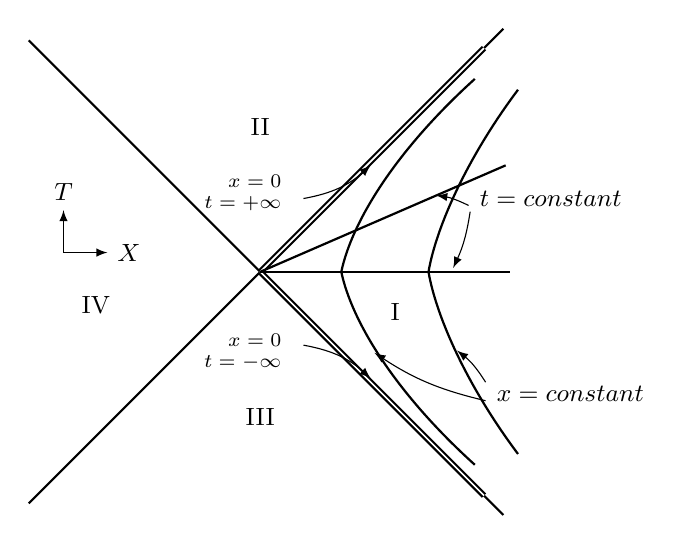
\begin{tikzpicture}[scale=.98,>=latex,font=\small]
  \coordinate (O) at (0,0);
  \draw[thick] (-3.0,-3.0) -- (3.15,3.15);
  \draw[thick] (-3.0,3.0) -- (3.15,-3.15);
  \draw[thick,double] (0,0) -- (2.9,2.9);
  \draw[thick,double] (0,0) -- (2.9,-2.9);
  \node at (1.75,-.52) {I};
  \node at (0,1.88) {II};
  \node at (0,-1.88) {III};
  \node at (-2.13,-.43) {IV};
  % Curves x=constant are right-opening hyperbolae.  Two members of the
  % family are shown, as in the source, together with two t=constant rays.
  \draw[thick] (2.78,-2.50)
    .. controls (1.72,-1.54) and (1.18,-.62) .. (1.05,0)
    .. controls (1.18,.62) and (1.72,1.54) .. (2.78,2.50);
  \draw[thick] (3.34,-2.36)
    .. controls (2.68,-1.48) and (2.28,-.58) .. (2.18,0)
    .. controls (2.28,.58) and (2.68,1.48) .. (3.34,2.36);
  \draw[thick] (0,0) -- (3.24,0);
  \draw[thick] (0,0) -- (3.18,1.38);
  \node[right] at (2.94,-1.58) {\(x=\text{constant}\)};
  \draw[->] (2.92,-1.43) to[bend right=10] (2.55,-1.02);
  \draw[->] (2.92,-1.67) to[bend left=10] (1.48,-1.05);
  \node[right] at (2.72,.94) {\(t=\text{constant}\)};
  \draw[->] (2.70,.86) to[bend right=9] (2.28,.99);
  \draw[->] (2.72,.78) to[bend left=8] (2.50,.05);
  \draw[->] (.56,.95) to[bend right=16] (1.43,1.38);
  \node[font=\scriptsize,left] at (.40,1.18) {\(x=0\)};
  \node[font=\scriptsize,left] at (.40,.89) {\(t=+\infty\)};
  \draw[->] (.56,-.95) to[bend left=16] (1.43,-1.38);
  \node[font=\scriptsize,left] at (.40,-.89) {\(x=0\)};
  \node[font=\scriptsize,left] at (.40,-1.18) {\(t=-\infty\)};
  \draw[->] (-2.55,.25) -- (-2.55,.80) node[above] {\(T\)};
  \draw[->] (-2.55,.25) -- (-1.98,.25) node[right] {\(X\)};
\end{tikzpicture}
\caption{Rindler spacetime, displayed as the wedge, I, of two-dimensional
Minkowski spacetime.}
\label{fig:6.8}
\end{figure}
\endgroup


Note that the time translation symmetry of the Rindler metric,
Eq.~\eqref{eq:6.4.3}, really corresponds to the boost symmetry of Minkowski
spacetime. The observers at constant \(x\) undergo the uniform acceleration
\(a=1/x\), which diverges as \(x\to0\). It is easy to check that static observers
in the Schwarzschild spacetime must undergo a proper acceleration in order to
stand still in the gravitational field given by
\(a=(1-2M/r)^{-1/2}M/r^2\), which diverges as \(r\to2M\). Thus, the behavior of
the Schwarzschild time coordinate as \(r\to2M\) is analogous to the behavior of
the Rindler time coordinate as \(x\to0\). (Indeed, the mathematical analogy
between the two metrics could be made more manifest by introducing a new space
coordinate \(y=x^2\) to put the Rindler metric in the form
\(ds^2=-y\,dt^2+4y^{-1}dy^2\).) Therefore, it should not be surprising that the
coordinate singularity of the Schwarzschild spacetime at \(r=2M\) is closely
analogous to that of the Rindler spacetime, as we now shall show.

The Schwarzschild spacetime is, of course, four-dimensional, but, because of the
spherical symmetry, only the two-dimensional \(r\)-\(t\) part of the metric is of
importance for analyzing the nature of the singularity at \(r=2M\). Hence, we
shall study the two-dimensional metric
\begin{equation}
  ds^2=-\left(1-\frac{2M}{r}\right)dt^2+
  \left(1-\frac{2M}{r}\right)^{-1}dr^2.
  \tag{6.4.16}\label{eq:6.4.16}
\end{equation}
We apply the two-dimensional method described above, using the outgoing and
ingoing radial null geodesics of the Schwarzschild spacetime. The null condition,
analogous to Eq.~\eqref{eq:6.4.4}, is
\begin{equation}
  0=g_{ab}k^ak^b
  =-\left(1-\frac{2M}{r}\right)\dot t^2+
  \left(1-\frac{2M}{r}\right)^{-1}\dot r^2,
  \tag{6.4.17}\label{eq:6.4.17}
\end{equation}
which implies
\begin{equation}
  (dt/dr)^2=\left(\frac{r}{r-2M}\right)^2.
  \tag{6.4.18}\label{eq:6.4.18}
\end{equation}
Thus, the radial null geodesics of Schwarzschild satisfy
\begin{equation}
  t=\pm r_*+\text{constant},
  \tag{6.4.19}\label{eq:6.4.19}
\end{equation}
where the Regge--Wheeler tortoise coordinate \(r_*\) is defined by
\begin{equation}
  r_*=r+2M\ln(r/2M-1),
  \tag{6.4.20}\label{eq:6.4.20}
\end{equation}
so that \(dr_*/dr=(1-2M/r)^{-1}\). We define the null coordinates \(u,v\) by
\begin{align}
  u&=t-r_*,
  &&\tag{6.4.21}\label{eq:6.4.21}\\
  v&=t+r_*.
  &&\tag{6.4.22}\label{eq:6.4.22}
\end{align}
In these coordinates,\footnote{The hybrid coordinates \((u,r)\) or \((v,r)\)
are known as Eddington--Finkelstein coordinates (Eddington 1924; Finkelstein
1958).} the metric \eqref{eq:6.4.16} takes the form
\begin{equation}
  ds^2=-\left(1-\frac{2M}{r}\right)du\,dv,
  \tag{6.4.23}\label{eq:6.4.23}
\end{equation}
where \(r\) is now viewed as a function of \(u\) and \(v\), defined implicitly by
\begin{equation}
  r+2M\ln\left(\frac{r}{2M}-1\right)=r_*=\frac{v-u}{2}.
  \tag{6.4.24}\label{eq:6.4.24}
\end{equation}
Using Eq.~\eqref{eq:6.4.24}, we can rewrite Eq.~\eqref{eq:6.4.23} as
\begin{equation}
  ds^2=-\frac{2Me^{-r/2M}}{r}e^{(v-u)/4M}\,du\,dv,
  \tag{6.4.25}\label{eq:6.4.25}
\end{equation}
where we have factored the metric components into a piece,
\(e^{-r/2M}/r\), which is nonsingular as \(r\to2M\), i.e., as \(u\to\infty\)
or \(v\to-\infty\), times a piece with simple \(u\) and \(v\) dependence.
Comparison with the Rindler case, Eq.~\eqref{eq:6.4.9} (or calculation of the
affine parameter along the null geodesics) suggests that we define new
coordinates \(U\) and \(V\) by
\begin{align}
  U&=-e^{-u/4M},
  &&\tag{6.4.26}\label{eq:6.4.26}\\
  V&=e^{v/4M},
  &&\tag{6.4.27}\label{eq:6.4.27}
\end{align}
in terms of which the metric becomes
\begin{equation}
  ds^2=-\frac{32M^3e^{-r/2M}}{r}\,dU\,dV.
  \tag{6.4.28}\label{eq:6.4.28}
\end{equation}
There is now no longer a singularity at \(r=2M\), i.e., at \(U=0\) or \(V=0\),
and thus we can extend the Schwarzschild solution by allowing \(U\) and \(V\) to
take on all values compatible with \(r>0\). The singularity which persists at
\(r=0\) is physical---as mentioned above, the curvature scalar
\(R_{abcd}R^{abcd}\) blows up there---so it cannot be eliminated by a further
coordinate transformation.

If we make the final transformation \(T=(U+V)/2\), \(X=(V-U)/2\), the full
Schwarzschild metric takes the final form given by Kruskal (1960) (see also
Szekeres 1960),
\begin{equation}
  ds^2=\frac{32M^3e^{-r/2M}}{r}(-dT^2+dX^2)
  +r^2(d\theta^2+\sin^2\theta\,d\phi^2).
  \tag{6.4.29}\label{eq:6.4.29}
\end{equation}
The relation between the old coordinates \((t,r)\) and the new coordinates
\((T,X)\) is given by
\begin{equation}
  \left(\frac{r}{2M}-1\right)e^{r/2M}=X^2-T^2,
  \tag{6.4.30}\label{eq:6.4.30}
\end{equation}
and
\begin{equation}
  \frac{t}{2M}=\ln\left(\frac{T+X}{X-T}\right)
  =2\tanh^{-1}(T/X),
  \tag{6.4.31}\label{eq:6.4.31}
\end{equation}
and in Eq.~\eqref{eq:6.4.29}, \(r\) is to be viewed as the function of \(X\) and
\(T\) defined by Eq.~\eqref{eq:6.4.30}. The allowed range of the coordinates
\(X\) and \(T\) is given by the condition \(r>0\), which yields
\begin{equation}
  X^2-T^2>-1.
  \tag{6.4.32}\label{eq:6.4.32}
\end{equation}

A spacetime diagram for the Kruskal extension is shown in Figure~\ref{fig:6.9}.
The causal structure of the extended Schwarzschild spacetime is easily seen from
the diagram since, by construction, the radial null geodesics are \(45^\circ\)
lines in Kruskal coordinates. The Kruskal extension is remarkably similar to the
extension of the Rindler spacetime, the major differences being (1) the
Schwarzschild spacetime is four-dimensional, so each point in
Figure~\ref{fig:6.9} really represents a two-dimensional sphere of radius \(r\)
and (2) there are physical singularities in the extended region at
\(X=\pm(T^2-1)^{1/2}\), as shown. Note that the singularities at \(r=0\) have a
spacelike character and exist in the future of region II and the past of region
III, rather than corresponding to a timelike line at the origin of coordinates as
a naive interpretation of the Schwarzschild coordinates \((t,r)\) might have
suggested. The bad behavior of the coordinates \((t,r)\) can also be seen in the
Kruskal diagram. From Eq.~\eqref{eq:6.4.30} we see that \(\nabla_a r=0\) at
\(X=T=0\), and it is not difficult to verify that the static Killing field
\(\xi^a\) vanishes there also. Note also that \(\nabla_a r\) and \(\xi^a\) become
collinear along the null lines \(X=\pm T\). The vanishing of \(\xi^a\) at
\(X=T=0\) leads to a mislabeling of the lines \(X=\pm T\) as
\(t=\pm\infty\) analogous to the behavior of the \(t\)-coordinate in Rindler
spacetime. Note, however, that although the Kruskal coordinates are very
convenient for analyzing the strong field region of the Schwarzschild geometry,
they are not convenient for analyzing the asymptotically flat region,
\(r\to\infty\).
% Source: Wald GR, physical PDF p. 167
%         (printed p. 154).
% Coverage: Figure 6.9, the Kruskal extension of Schwarzschild spacetime.
% Figures/tables/footnotes: Figure 6.9; no tables or footnotes.
% Status: source-reviewed and compile-clean.
% Uncertainties: none.
\begingroup
\renewcommand{\thefigure}{6.9}
\begin{figure}[htbp]
\centering
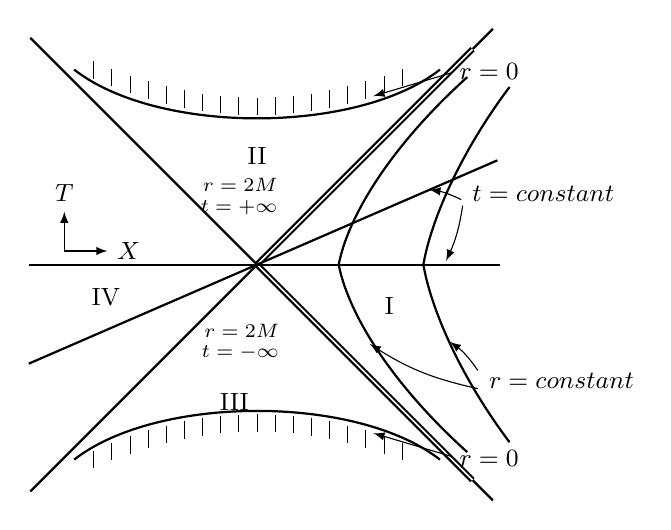
\begin{tikzpicture}[scale=.96,>=latex,font=\small]
  \draw[thick] (-3.0,-3.0) -- (3.12,3.12);
  \draw[thick] (-3.0,3.0) -- (3.12,-3.12);
  \draw[thick,double] (0,0) -- (2.85,2.85);
  \draw[thick,double] (0,0) -- (2.85,-2.85);
  \draw[thick] (2.78,-2.48)
    .. controls (1.74,-1.54) and (1.20,-.62) .. (1.08,0)
    .. controls (1.20,.62) and (1.74,1.54) .. (2.78,2.48);
  \draw[thick] (3.34,-2.35)
    .. controls (2.68,-1.47) and (2.30,-.58) .. (2.20,0)
    .. controls (2.30,.58) and (2.68,1.47) .. (3.34,2.35);
  \draw[thick] (-3.02,0) -- (3.22,0);
  \draw[thick] (-3.02,-1.31) -- (3.18,1.38);
  \draw[thick] (-2.42,2.58) .. controls (-1.32,1.72) and (1.32,1.72) .. (2.42,2.58);
  \draw[thick] (-2.42,-2.58) .. controls (-1.32,-1.72) and (1.32,-1.72) .. (2.42,-2.58);
  \foreach \x in {-2.16,-1.92,...,2.16} {
    \draw (\x,{1.98+.103*\x*\x}) -- ++(0,.23);
    \draw (\x,{-1.98-.103*\x*\x}) -- ++(0,-.23);
  }
  \node at (1.75,-.55) {I};
  \node at (0,1.44) {II};
  \node at (-.30,-1.82) {III};
  \node at (-2.00,-.43) {IV};
  \node[font=\scriptsize,left] at (.40,1.05) {\(r=2M\)};
  \node[font=\scriptsize,left] at (.40,.76) {\(t=+\infty\)};
  \node[font=\scriptsize,left] at (.42,-.88) {\(r=2M\)};
  \node[font=\scriptsize,left] at (.42,-1.17) {\(t=-\infty\)};
  \draw[->] (2.58,2.54) -- (1.54,2.23);
  \node[right] at (2.55,2.56) {\(r=0\)};
  \draw[->] (2.58,-2.54) -- (1.54,-2.23);
  \node[right] at (2.55,-2.56) {\(r=0\)};
  \node[right] at (2.94,-1.54) {\(r=\text{constant}\)};
  \draw[->] (2.92,-1.40) to[bend right=10] (2.55,-1.02);
  \draw[->] (2.92,-1.64) to[bend left=10] (1.49,-1.05);
  \node[right] at (2.72,.94) {\(t=\text{constant}\)};
  \draw[->] (2.70,.86) to[bend right=9] (2.28,.99);
  \draw[->] (2.72,.78) to[bend left=8] (2.50,.05);
  \draw[->] (-2.55,.18) -- (-2.55,.70) node[above] {\(T\)};
  \draw[->] (-2.55,.18) -- (-1.98,.18) node[right] {\(X\)};
\end{tikzpicture}
\caption{The Kruskal extension of Schwarzschild spacetime.}
\label{fig:6.9}
\end{figure}
\endgroup


The extended Schwarzschild spacetime has a rather surprising structure. The
region I of Figure~\ref{fig:6.9} corresponds to the original region \(r>2M\) of
the Schwarzschild solution, and can be interpreted physically as representing the
exterior gravitational field of a spherical body. However, a radially infalling
observer in region I will cross the null line \(X=T\) and enter region II. Once
this observer has entered region II, he can never escape from it. Within a finite
proper time (see problem~6) he will unavoidably fall into the singularity at
\(X=(T^2-1)^{1/2}\) and, indeed, any light signal he sends from region II will
remain in region II and also will fall into the singularity. For this reason,
region II is referred to as a \emph{black hole}. (A general definition of the
notion of a black hole will be given in Chapter~12.) Region III has exactly the
time reversed properties of region II, and is referred to as a \emph{white hole}.
Any observer present in region III must have originated in the spacetime
singularity at \(X=-(T^2-1)^{1/2}\) and, within a finite time, must leave region
III. Finally region IV has properties identical to the original region I. It
represents another asymptotically flat region of spacetime which lies inside the
radius \(r=2M\). How this can occur is best illustrated by examining the geometry
of the spacelike surface \(T=0\), which is shown in Figure~\ref{fig:6.10}. Note,
however, that an observer in region I cannot communicate with any observer in
region IV; as seen from Figure~\ref{fig:6.9}, a light signal sent from region I
toward region IV will instead go into the black hole and be swallowed up by the
spacetime singularity.
% Source: Wald GR, physical PDF p. 168
%         (printed p. 155).
% Coverage: Figure 6.10, spatial geometry of the \(t=0\) Schwarzschild hypersurface.
% Figures/tables/footnotes: Figure 6.10; no tables or footnotes.
% Status: source-reviewed and compile-clean.
% Uncertainties: none.
\begingroup
\renewcommand{\thefigure}{6.10}
\begin{figure}[htbp]
\centering
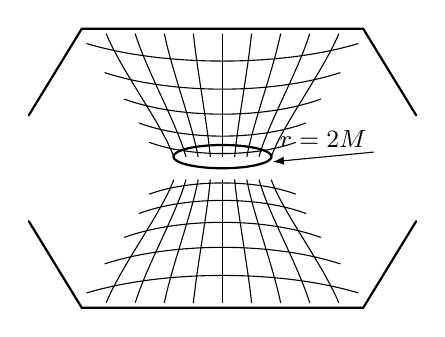
\begin{tikzpicture}[scale=.82,>=latex,font=\small,line cap=round]
  % Two asymptotically flat ends joined by the minimum-area throat.
  \draw[thick] (-3.0,.82) -- (-2.18,2.16) -- (2.18,2.16) -- (3.0,.82);
  \draw[thick] (-3.0,-.82) -- (-2.18,-2.16) -- (2.18,-2.16) -- (3.0,-.82);
  \foreach \x in {-1.8,-1.35,-.9,-.45,0,.45,.9,1.35,1.8} {
    \draw[thin] (\x,2.08) .. controls ({.86*\x},1.48) and ({.52*\x},.68) .. ({.42*\x},.18);
    \draw[thin] ({.42*\x},-.18) .. controls ({.52*\x},-.68) and ({.86*\x},-1.48) .. (\x,-2.08);
  }
  \draw[thin] (-2.10,1.93) .. controls (-.90,1.57) and (.90,1.57) .. (2.10,1.93);
  \draw[thin] (-1.82,1.48) .. controls (-.78,1.14) and (.78,1.14) .. (1.82,1.48);
  \draw[thin] (-1.52,1.07) .. controls (-.66,.76) and (.66,.76) .. (1.52,1.07);
  \draw[thin] (-1.29,.70) .. controls (-.57,.43) and (.57,.43) .. (1.29,.70);
  \draw[thin] (-1.13,.40) .. controls (-.51,.17) and (.51,.17) .. (1.13,.40);
  \draw[thin] (-1.13,-.40) .. controls (-.51,-.17) and (.51,-.17) .. (1.13,-.40);
  \draw[thin] (-1.29,-.70) .. controls (-.57,-.43) and (.57,-.43) .. (1.29,-.70);
  \draw[thin] (-1.52,-1.07) .. controls (-.66,-.76) and (.66,-.76) .. (1.52,-1.07);
  \draw[thin] (-1.82,-1.48) .. controls (-.78,-1.14) and (.78,-1.14) .. (1.82,-1.48);
  \draw[thin] (-2.10,-1.93) .. controls (-.90,-1.57) and (.90,-1.57) .. (2.10,-1.93);
  \draw[thick] (-.76,.18) arc[start angle=180,end angle=360,x radius=.76,y radius=.18];
  \draw[thick] (-.76,.18) arc[start angle=180,end angle=0,x radius=.76,y radius=.18];
  \draw[->] (2.34,.25) -- (.78,.10) node[midway,above] {\(r=2M\)};
\end{tikzpicture}
\caption{The spatial geometry of the hypersurface \(t=0\) of the Schwarzschild
spacetime, shown as it would look if it were embedded in flat space. (One
dimension is suppressed, i.e., the topology of the hypersurface is
\(\mathbb R\times S^2\), not \(\mathbb R\times S^1\), so each circle---such as
the one shown at \(r=2M\)---really represents a two-sphere.) The portion of the
surface lying above the throat at \(r=2M\) in the figure corresponds to the
portion lying in region I of Figure~\ref{fig:6.9}; the portion below \(r=2M\)
lies in region IV of Figure~\ref{fig:6.9}.}
\label{fig:6.10}
\end{figure}
\endgroup


How much of this picture of the extended Schwarzschild solution should we take
seriously? The extended Schwarzschild solution is, of course, a perfectly valid
solution of the vacuum Einstein equation, and as such, represents a possible
structure for spacetime in general relativity. However, in order to produce the
fully extended Schwarzschild solution, we must start with two asymptotically flat
regions of spacetime together with an initial singularity in the region III which
connects them. There is no reason to believe that the initial configuration of any
region of our universe corresponds to these initial conditions, so there is no
reason to believe that any region of our universe corresponds to the fully extended
Schwarzschild solution (although, of course, this possibility cannot easily be
ruled out). However, as discussed in Section~\ref{sec:6.2}, sufficiently massive
bodies will undergo complete gravitational collapse. The interior metric of these
bodies will not be the Schwarzschild metric since \(T_{ab}\ne0\) there, but at all
stages of the collapse the metric outside a spherical body will be the
Schwarzschild metric, since, as mentioned at the end of Section~\ref{sec:6.1}, it
is the only spherically symmetric vacuum solution of Einstein's equation.
Therefore, the spacetime geometry corresponding to the gravitational collapse of a
spherical body will be as shown in Figure~\ref{fig:6.11}. All of regions III and
IV (as well as parts of regions I and II) will be covered up by the matter and
thus replaced by a normal spacetime region. However, a spacetime region
corresponding to region II of the extended vacuum Schwarzschild spacetime will be
produced when the radial coordinate of the collapsing body becomes less than
\(2M\). Another representation of the spacetime geometry resulting from spherical
collapse is shown in Figure~\ref{fig:6.12}.
% Source: Wald GR, physical PDF p. 169
%         (printed p. 156).
% Coverage: Figure 6.11, complete gravitational collapse.
% Figures/tables/footnotes: Figure 6.11; no tables or footnotes.
% Status: source-reviewed and compile-clean.
% Uncertainties: none.
\begingroup
\renewcommand{\thefigure}{6.11}
\begin{figure}[htbp]
\centering
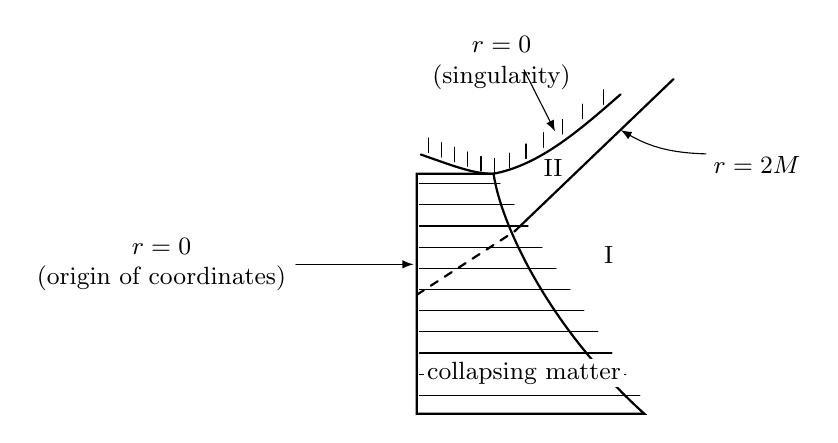
\begin{tikzpicture}[scale=.84,>=latex,font=\small,line cap=round]
  % World tube of the matter: the left edge is the regular center r=0 and
  % the right edge shrinks as the body collapses.
  \draw[thick] (-1.72,-2.58) -- (-1.72,1.05) -- (-.56,1.05)
    .. controls (-.45,.28) and (.28,-1.28) .. (1.72,-2.58) -- cycle;
  \foreach \y in {-2.30,-1.98,-1.66,-1.34,-1.02,-.70,-.38,-.06,.26,.58,.90} {
    \draw[thin] (-1.68,\y) -- ({-.56+.66*(1.05-\y)},\y);
  }
  % Event horizon: dashed while it lies inside the matter, solid outside.
  \draw[dashed,thick] (-1.72,-.78) -- (-.24,.18);
  \draw[thick] (-.24,.18) -- (2.16,2.48);
  % The future spacelike singularity.
  \draw[thick] (-1.66,1.34) .. controls (-1.20,1.18) and (-.85,1.04) .. (-.56,1.05)
    .. controls (.12,1.18) and (.70,1.67) .. (1.36,2.25);
  \foreach \x/\y in {-1.55/1.37,-1.35/1.30,-1.15/1.23,-.95/1.16,-.75/1.09,
      -.55/1.06,-.32/1.14,-.07/1.28,.20/1.45,.48/1.65,.78/1.88,1.10/2.10} {
    \draw (\x,\y) -- ++(0,.22);
  }
  \draw[->] (2.65,1.35) to[bend left=14] (1.36,1.71);
  \node[right] at (2.62,1.18) {\(r=2M\)};
  \draw[->] (-3.55,-.32) -- (-1.77,-.32);
  \node[align=center,anchor=east] at (-3.55,-.32) {\(r=0\)\\(origin of coordinates)};
  \draw[->] (-.10,2.62) -- (.37,1.69);
  \node[align=center] at (-.44,2.72) {\(r=0\)\\(singularity)};
  \node[fill=white,inner sep=1pt] at (-.10,-1.96) {collapsing matter};
  \node at (1.18,-.18) {I};
  \node at (.34,1.13) {II};
\end{tikzpicture}
\caption{The spacetime resulting from the complete gravitational collapse of a
spherical body. All of regions III and IV of the extended Schwarzschild
spacetime (Figure~\ref{fig:6.9}) are covered up by the collapsing matter.
However, part of the black hole region II is produced.}
\label{fig:6.11}
\end{figure}
\endgroup

% Source: Wald GR, physical PDF p. 170
%         (printed p. 157).
% Coverage: Figure 6.12, another representation of the Figure 6.11 spacetime.
% Figures/tables/footnotes: Figure 6.12; no tables or footnotes.
% Status: source-reviewed and compile-clean.
% Uncertainties: none.
\begingroup
\renewcommand{\thefigure}{6.12}
\begin{figure}[htbp]
\centering
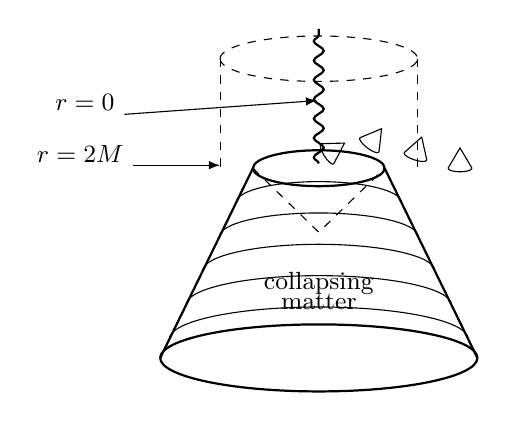
\begin{tikzpicture}[scale=.76,>=latex,font=\small]
  \draw[dashed] (-1.65,2.65) arc[start angle=180,end angle=360,x radius=1.65,y radius=.38];
  \draw[dashed] (-1.65,2.65) arc[start angle=180,end angle=0,x radius=1.65,y radius=.38];
  \draw[dashed] (-1.65,2.65) -- (-1.65,.75);
  \draw[dashed] (1.65,2.65) -- (1.65,.75);
  \draw[thick] (-2.65,-2.35) arc[start angle=180,end angle=360,x radius=2.65,y radius=.56];
  \draw[thick] (-2.65,-2.35) arc[start angle=180,end angle=0,x radius=2.65,y radius=.56];
  \draw[thick] (-2.65,-2.35) -- (-1.10,.82);
  \draw[thick] (2.65,-2.35) -- (1.10,.82);
  \draw[thick] (-1.10,.82) arc[start angle=180,end angle=360,x radius=1.10,y radius=.30];
  \draw[thick] (-1.10,.82) arc[start angle=180,end angle=0,x radius=1.10,y radius=.30];
  \foreach \t in {.1,.28,.46,.64,.82} {
    \draw[thin] ({-2.65+1.55*\t},{-2.35+3.17*\t}) arc[start angle=180,end angle=0,
      x radius={2.65-1.55*\t},y radius={.56-.26*\t}];
  }
  \draw[thick,decorate,decoration={snake,amplitude=1.8pt,segment length=7pt}]
    (0,.90) -- (0,3.15);
  \foreach \x/\y/\a in {.43/1.24/-58,1.05/1.48/-37,1.72/1.34/-18,2.36/1.16/0} {
    \begin{scope}[shift={(\x,\y)},rotate=\a]
      \draw[thin] (-.20,-.34) -- (0,0) -- (.20,-.34);
      \draw[thin] (-.20,-.34) arc[start angle=180,end angle=360,x radius=.20,y radius=.06];
    \end{scope}
  }
  \draw[dashed] (-1.10,.82) -- (0,-.25) -- (1.10,.82);
  \node at (0,-1.10) {collapsing};
  \node at (0,-1.42) {matter};
  \draw[->] (-3.25,1.72) -- (-.03,1.95);
  \node[left] at (-3.25,1.92) {\(r=0\)};
  \draw[->] (-3.10,.87) -- (-1.65,.87);
  \node[left] at (-3.10,1.06) {\(r=2M\)};
\end{tikzpicture}
\caption{Another representation of the spacetime of Figure~\ref{fig:6.11}.
Here, one of the two suppressed spatial dimensions is restored, so each of the
circles shown on the collapsing body corresponds to the 2-sphere surface of the
body at an instant of time. However, the light cones no longer are represented by
\(45^\circ\) lines. Indeed, the spacelike nature of the singularity and the
inevitable capture by the singularity of any particle or light ray in the region
\(r<2M\) is illustrated here by the tipping over of the future light cones in the
strong field region.}
\label{fig:6.12}
\end{figure}
\endgroup


Thus, regions III and IV of the extended Schwarzschild solution are probably
unphysical, but region II is of great physical importance: \emph{The complete
gravitational collapse of a spherical body always produces a Schwarzschild black
hole region of spacetime.}
